%
%  Thesis Vorlage für die Hochschule Heilbronn
%
%  Created by Prof. Dr. Detlef Stern on 2010-08-14.
%  Updated by Valentin Weber on 2020-10-05.
%  Copyright (c) 2020 . All rights reserved.
%
\documentclass[12pt,toc=bib,toc=listof]{scrreprt}
\usepackage[ngerman,provide=*]{babel}
\usepackage[utf8]{inputenc}
\usepackage[T1]{fontenc}
\usepackage{lmodern}
\usepackage{setspace}
\usepackage{geometry}
\usepackage{cite}
\usepackage[authoryear]{natbib}
\usepackage{chngcntr}
\usepackage{float}
\usepackage{fancyvrb}
\usepackage{amsmath}
\counterwithout{footnote}{chapter}
\counterwithout{figure}{chapter}

\usepackage{pgfplots}
\pgfplotsset{compat=1.18}
\usepgfplotslibrary{statistics}

\usepackage{hyperref}
\hypersetup{
  ,colorlinks=true
  ,linkcolor=black
  ,citecolor=black
  ,filecolor=black
  ,urlcolor=black
  }

\newcommand{\thesis}{Bachelorthesis}
\newcommand{\hhnsubject}{Angewandte Informatik}
\newcommand{\hhnsubjectnum}{SPO1a}
\newcommand{\hhnlecturer}{Prof. Dr. Fankhauser}

\newcommand{\reprttopic}{GraphQL und REST im Kontext relationaler und graphbasierter Datenbanken hinsichtlich Latenz bei unterschiedlichen Anfragekomplexitäten}
\newcommand{\reprtstudentname}{Robin Hefner}
\newcommand{\reprtstudentid}{206488}
\urldef{\reprtstudentmail}\url{rohefner@stud.hs-heilbronn.de}

\usepackage[headsepline]{scrlayer-scrpage}
\pagestyle{scrheadings}
\clearscrheadfoot
\ihead{\reprttopic}
\ohead{\raisebox{-10pt}{\pagemark}}
\renewcommand*{\chapterpagestyle}{scrheadings}
\renewcommand*{\chapterheadstartvskip}{}

% Deckblatt Definitionen (begin)
\titlehead{\flushright\includegraphics{./Illustrations/hhn.png}}
\subject{{\thesis \\\hhnsubject{} (\hhnsubjectnum{})}}
\title{\reprttopic}
\author{\reprtstudentname\footnote{\reprtstudentid, \reprtstudentmail}}
%% Datum nie auf einen festen Wert setzen
\publishers{Eingereicht bei \hhnlecturer}
% Deckblatt Definitionen (end)

\begin{document}
\pagenumbering{Roman} 
\selectlanguage{ngerman}
\maketitle
\newpage
\newgeometry{left=30mm, top=25mm, right=15mm, bottom=25mm}
\tableofcontents
\newpage
\addchap{Abkürzungsverzeichnis} % (fold)
\label{sec:abkuerzungsverzeichnis}

\begin{description}
  	\item[API:] Application Programming Interface
	\item[HTTP:] Hypertext Transfer Protocol
	\item[REST:] Representational State Transfer
	\item[RPC:]Remote Prodecdure Call
	\item[SOAP:]Simple Object Access Protocol
	\item[URL:] Uniform Resource Locator
\end{description}

% chapter abkuerzungsverzeichnis (end)

\newpage
\listoffigures
\newpage

\addchap{Abstract} % (fold)
\label{sec:abstract}
This thesis analyses the performance of GraphQL and REST in the context of relational and graph-based databases in terms of latency for different query complexities. The aim of the analysis was to evaluate the advantages and disadvantages of both API technologies and to understand the interactions with the underlying database architectures.
\newline
\noindent
The results show that GraphQL offers clear advantages for complex queries, as it reduces the number of API calls through client-driven data queries.
For bulk queries with large amounts of data, REST was able to achieve better response times, while GraphQL was superior for hierarchical and flexible queries.
In terms of database technologies, relational databases proved to be efficient with structured data and low branching, while graph databases were particularly convincing with highly networked data and high query complexity thanks to their traversal mechanisms.
\newline
\noindent
The combination of GraphQL and graph databases showed a significant reduction in latency in complex scenarios. For simpler queries, GraphQL was also able to achieve better latencies with a relational database than a comparable REST API. The findings provide practical information for selecting the optimal API and database technology and offer guidance for the development of high-performance and scalable systems.
\newline
\noindent
\textbf{Keywords:} REST, GraphQL, API, relational database, graph database
% chapter abstract (end)
\newpage
\addchap{Zusammenfassung} % (fold)
\label{sec:zusammenfassung}
Die vorliegende Arbeit untersucht die Performance von GraphQL und REST im Kontext von relationalen und graphbasierten Datenbanken hinsichtlich der Latenz bei unterschiedlichen Anfragekomplexitäten. Ziel der Analyse war es, die Vor- und Nachteile beider API-Technologien zu bewerten und die Wechselwirkungen mit den zugrunde liegenden Datenbankarchitekturen zu verstehen.
\newline
\noindent
Die Ergebnisse zeigen, dass GraphQL bei komplexen Abfragen deutliche Vorteile bietet, da es durch clientgesteuerte Datenabfragen die Anzahl der API-Aufrufe reduziert.
Bei Bulk-Abfragen mit großen Datenmengen konnte REST bessere Antwortzeiten erzielen, während GraphQL bei hierarchischen und flexiblen Abfragen überlegen war.
Hinsichtlich der Datenbanktechnologien erwiesen sich relationale Datenbanken als effizient bei strukturierten Daten und geringen Verzweigungen, während Graphdatenbanken durch ihre Traversal-Mechanismen besonders bei stark vernetzten Daten und hohen Abfragekomplexitäten überzeugten.
\newline
\noindent
Die Kombination aus GraphQL und Graphdatenbanken zeigte eine signifikante Reduzierung der Latenz bei komplexen Szenarien. Bei einfacheren Anfragen konnte GraphQL ebenfalls mit einer relationalen Datenbank bessere LAtenzen erzielen als eine vergleichbare REST API. Die gewonnenen Erkenntnisse liefern praxisrelevante Hinweise für die Auswahl der optimalen API- und Datenbanktechnologie und bieten Orientierungshilfen für die Entwicklung leistungsstarker und skalierbarer Systeme.
\newline
\noindent
\textbf{Stichwörter:} REST, GraphQL, API, relationale Datenbank, Graphdatenbank
% chapter zusammenfassung (end)

\onehalfspacing

% report (begin)
\numberwithin{figure}{chapter}
\chapter{Einleitung} % (fold)
\pagenumbering{arabic}
\label{sec:einleitung}

\section{Motivation} % (fold)
\label{sec:motivation}
In der modernen Softwareentwicklung spielen APIs (Application Programming Interfaces) eine entscheidende Rolle bei der Integration und Kommunikation zwischen verschiedenen Diensten und Anwendungen. Traditionell wurde REST (Representational State Transfer) als Standard für die Erstellung und Nutzung von APIs verwendet. Mit der Einführung und zunehmenden Verbreitung von GraphQL, einer Abfragesprache für APIs, die von Facebook entwickelt wurde, stehen Entwickler nun vor der Wahl zwischen diesen beiden Ansätzen. Die Wahl zwischen REST und GraphQL hat signifikante Auswirkungen auf die Entwicklung und den Betrieb der Anwendung. Unternehmen
müssen eine fundierte Entscheidung treffen, welche Technologie besser zu ihren Anforderungen, im Hinblick auf Leistungsfähigkeit und Anpassungsfähigkeit, passt.

% section motivation (end)

\section{Forschungsfragen} % (fold)
\label{sec:forschungsfragen}
Nachfolgend sollen die Forschungsfragen vorgestellt werden, die aus der Motivation abgeleitet wurden. Diese dienen als Grundlage der Forschung für diese Thesis.
\begin{itemize}
	\item \textbf{FF-1: Wie unterscheiden sich GraphQL und REST hinsichtlich der Anfrage- und Antwortzeiten unter verschiedenen Lastbedingungen und Anfragenkomplexitäten ?}  Diese Frage zielt darauf ab, die Performance beider Systeme unter variablen Bedingungen zu vergleichen. Beispielsweise könnte untersucht werden, wie schnell eine API auf eine einfache Datenabfrage reagiert, im Vergleich zu einer komplexeren, die mehrere Abhängigkeiten involviert. Diese Untersuchung könnte Einblicke in die Effizienz der beiden Technologien bieten und somit als Entscheidungshilfe für Entwickler dienen, die die beste Lösung für ihre spezifischen Bedürfnisse auswählen möchten.
	\item \textbf{FF-2: Inwiefern bieten GraphQL und REST unterschiedliche Möglichkeiten zur Abfrageanpassung?} Diese Frage beleuchtet die Flexibilität beider Systeme in Bezug auf die Individualisierung von Datenabfragen. Während REST traditionell durch feste Endpunkte gekennzeichnet ist, die jeweils eine bestimmte Datenstruktur zurückgeben, bietet GraphQL eine dynamischere Herangehensweise. Mit GraphQL können Clients genau die Daten anfordern, die sie benötigen, und keine zusätzlichen Informationen, was zu effizienteren Datenübertragungen führen kann. 

Diese Fähigkeit, Anfragen präzise anzupassen, könnte die Effizienz und Benutzerfreundlichkeit von Webanwendungen erheblich beeinflussen.
\end{itemize}
% section forschungsfragen (end)

\section{Vorgehensweise} % (fold)
\label{sec:vorgehensweise}

Für die Untersuchung werden sowohl theoretische Analysen als auch empirische Experimente durchgeführt. Im Rahmen der theoretischen Analyse erfolgt eine umfassende Literaturrecherche und die Analyse bestehender Studien zur Leistungsfähigkeit und Anpassungsfähigkeit von REST und GraphQL. Die empirischen Experimente umfassen die Implementierung von Beispiel-APIs mit beiden Technologien sowie die Durchführung von Leistungs- und Flexibilitätstests. Die Leistungstests konzentrieren sich auf das Messen der Latenz, des Durchsatzes und der Ressourcenauslastung bei verschiedenen Abfrageszenarien. Die Flexibilitätstests bewerten die Anpassungsfähigkeit der APIs an wechselnde Anforderungen und Schemaänderungen.


% section vorgehensweise (end)
% chapter einleitung (end)
\chapter{Grundlagen} % (fold)
\label{sec:grundlagen}
Die folgenden Abschnitte sollen die theoretischen Grundlagen vermitteln, die notwendig sind, um das Thema dieser Thesis zu betrachten. Die Konzepte, die hier beschrieben werden sind APIs, wie REST und GraphQL, als auch relationale und Graph Datenbanken.
\section{API} % (fold)
\label{sec:apigrundlagen}
Nachfolgend werden die Grundlagen von APIs thematisiert. Hierbei werden die grundlegenden Definitionen im Zusammenhang mit APIs und die verschiedenen Typen vorgestellt.
\subsection{Grundlegende Definition von API} % (fold)
\label{sec:grundlegendedefinitionvonapi}
Der Begriff \glqq API\grqq{}  steht für \glqq Application Programming Interface\grqq{}. Eine API bezeichnet eine Schnittstelle, welche Entwicklern den Zugriff auf Daten und Informationen ermöglicht. Bekannte Beispiele für häufig genutzte APIs sind die Twitter- und Facebook-APIs. Diese sind für Entwickler zugänglich und ermöglichen die Interaktion mit der Software von Twitter und Facebook. Zudem ermöglichen APIs die Kommunikation zwischen Anwendungen. Sie bieten den Anwendungen einen Weg, miteinander über das Netzwerk, überwiegend das Internet, in einer gemeinsamen Sprache zu kommunizieren. \citep{apistrategyguide}
%subsection grundlegendedefinitionvonapi (end)
\subsection{API Typen} % (fold)
\label{sec:apitypen}
APIs können anhand von Verfügbarkeit, Anwendungszweck oder der Spezifikation in verschiedene Typen eingeteilt werden.

\subsubsection{API Typen nach Verfügbarkeit} % (fold)
\label{sec:apitypenverfuegbarkeit}
Im Bezug auf Verfügbarkeit können APIs public (öffentlich), privat oder für Partner bereitgestellt werden. 
\begin{figure}[h!]
	\centering
	\includegraphics[scale=0.225]{Illustrations/apitypes.jpg}
	\caption{API Typen nach Verfügbarkeit \citep{graficapitypes}}
\end{figure}

\begin{itemize}
	\item \textbf{Public APIs:} Öffentliche APIs sind für jeden Entwickler bzw. jegliche Dritte verfügbar. Eine öffentliche API kann zu einer Steigerung der Markenbekanntheit beitragen und eröffnet bei einer Monetarisierung zusätzliche Einnahmequellen.\citep{apistrategyguide}
	\item \textbf{Privat APIs:} Dieser Typ erlaubt es Entwicklern, die innerhalb einer Firma tätig sind, die API zu nutzen, um interne Produkte, Systeme oder Apps zu integrieren. Des Weiteren können bei der Entwicklung neuer Systeme bereits vorhandene Ressourcen verwendet werden. Dadurch lassen sich die Kosten erheblich reduzieren und es entsteht eine größere Flexibilität. \citep{apistrategyguide}
	\item \textbf{Partner APIs:} Partner-APIs stellen eine Art Schnittstelle zwischen privaten und öffentlichen APIs dar. Ihr Zweck besteht darin, die Entwicklung von Unternehmensanwendungen zu fördern. Die Unternehmen haben dabei eine hohe Nutzerkontrolle.\citep{apistrategyguide}
\end{itemize}
%subsubsection apitypenverfuegbarkeit (end)

\subsubsection{API Typen nach Anwendungszweck} % (fold)
\label{sec:apitypenanwendungszweck}
\begin{itemize}
\item \textbf{Datenbanken APIs} ermöglichen die Kommunikation zwischen einer Datenbank und einer Anwendung die deren Daten benötigt. \citep{TUM}

\item \textbf{Betriebssystem APIs} definieren wie Ressourcen und Services von Betriebssystemen von einer Anwendung benutzt werden, die auf deren Daten zugreift. \citep{TUM}

\item \textbf{Remote APIs} definieren die Regeln, wie Anwendungen auf verschiedenen Host-Maschinen miteinander interagieren. \citep{TUM}

\item \textbf{Web APIs} sind die verbreitetsten APIs. Sie stellen Daten bereit und übermitteln diese zwischen Web-basierenden Systemen über eine Client-Server Verbindung. \citep{TUM}

\end{itemize}
%subsubsection apitypenanwendungszweck (end)

\subsubsection{API Typen nach Spezifikation/Protokoll} % (fold)
\label{sec:apitypenspezifikation}
Das Ziel der Spezifikation von APIs ist die Kommunikation zwischen verschiedenen Services zu standardisieren

\begin{itemize}

	\item \textbf{Remote Procedure Call (RPC)} stellt eine einfache und zugleich die älteste Form von Application Programming Interfaces dar. Ihr Zweck besteht in der Initiierung von Prozeduren auf unterschiedlichen Computern über das Netzwerk hinweg. Zu diesem Zweck übermittelt eine Anwendung eine oder mehrere Nachrichten an eine andere Anwendung, um eine Prozedur zu starten. Im Anschluss daran sendet die empfangende Anwendung dem Sender eine oder mehrere Nachrichten zurück, sobald die Prozedur abgeschlossen ist. Obwohl es konzeptionell einfach und leicht zu implementieren ist, gibt es eine Menge verschiedener und subtile Probleme, die zu unterschiedlichen RPC-Implementierungen führen.
	\citep{RPC}

	\item \textbf{Simple Object Access Protocol (SOAP)} stellt ein leichtgewichtiges Protokoll für den Austausch von Informationen in einer dezentralen, verteilten Umgebung dar. Es handelt sich um ein XML-basiertes Protokoll, welches aus drei Teilen besteht: einem Umschlag, welcher einen Rahmen für die Beschreibung des Inhalts einer Nachricht sowie ihrer Verarbeitung definiert, einer Reihe von Kodierungsregeln für die Darstellung von Instanzen anwendungsdefinierter Datentypen sowie einer Konvention für die Darstellung von Remote-Prozeduraufrufen und Antworten. SOAP kann potenziell in Kombination mit einer Vielzahl von anderen Protokollen verwendet werden.
	\citep{SOAP}

	\item \textbf{Representational State Transfer (REST)} wurde erstmals im Jahr 2000 in einer Dissertation von Roy Fielding beschrieben. Hierbei handelt es sich um einen Software-Architekturstil für APIs. REST basiert auf einer Ressourcenorientierung, bei der jede Entität als Ressource betrachtet und durch eine eindeutige Uniform Resource Locator (URL) identifiziert wird. Die Architektur basiert auf sechs grundlegenden Beschränkungen, darunter die Client-Server-Architektur, bei der Client und Server unabhängig voneinander agieren. Ein wesentliches Charakteristikum von REST ist die Zustandslosigkeit, d. h. jede Anfrage beinhaltet sämtliche für die Verarbeitung erforderlichen Informationen, wodurch die Interaktion zwischen Client und Server vereinfacht wird. Die Umsetzung der CRUD-Operationen (Create, Read, Update, Delete) erfolgt durch die HTTP-Methoden (POST, GET, PUT, DELETE). REST nutzt das in HTTP integrierte Caching, um die Antwortzeiten und die Leistung zu optimieren. Dabei besteht die Möglichkeit, Serverantworten als cachefähig oder nicht cachefähig zu kennzeichnen. Des Weiteren ist eine einheitliche Schnittstelle zu nennen, welche die Interaktionen zwischen unterschiedlichen Geräten und Anwendungen erleichtert und sichtbar macht. Darüber hinaus erfordert REST ein mehrschichtiges System, bei dem jede Komponente lediglich mit der unmittelbar vorgelagerten Schicht interagiert. Die Bereitstellung von ausführbarem Code durch den Server ist optional. RESTful APIs, die diesen Prinzipien folgen, nutzen HTTP-Anfragen, um Ressourcen effizient zu bearbeiten. \citep{Fielding2000}  \citep{graphqlreplacerest}

	\item \textbf{GraphQL} wurde 2012 von Facebook für den internen Gebrauch entwickelt. Im Jahr 2015 erfolgte die Veröffentlichung als Open-Source-Projekt für die Allgemeinheit. Das Kernkonzept von GraphQL basiert auf client-getriebenen Abfragen, bei denen der Client die Struktur der Daten präzise definiert und nur die erforderlichen Daten erhält. Dies resultiert in einer Reduktion von Datenübertragungen und ermöglicht effizientere Netzwerkaufrufe. Die hierarchische Struktur der Abfragen, welche die Graph-Struktur widerspiegelt, erlaubt eine intuitive Datenmodellierung. Die starke Typisierung in GraphQL wird durch ein Schema definiert, welches die Typen der Daten spezifiziert. Dadurch wird eine bessere Validierung und Dokumentation ermöglicht. Im Gegensatz zu REST, bei dem für verschiedene Operationen mehrere Endpunkte erforderlich sind, verwendet GraphQL lediglich einen einzigen Endpunkt für alle API-Abfragen.  \citep{graphqlreplacerest}

\end{itemize}
%subsubsection apitypenspezifikation (end)
%subsection apitypen (end)

% section apigrundlagen (end)

\section{Datenbank} % (fold)
\label{sec:datenbankGrundlagen}
Im Folgenden werden die Grundlagen von Datenbanken behandelt. Es werden grundlegende Definitionen im Zusammenhang mit Datenbanken und die verschiedenen Arten von Datenbanken vorgestellt.
\subsection{Definition Datenbank und Datenbank Management System} % (fold)
\label{sec:definitiondatenbank}
Eine Datenbank stellt eine Sammlung von Daten und Informationen dar, welche für einen einfachen Zugriff gespeichert und organisiert werden. Dies umfasst sowohl die Verwaltung als auch die Aktualisierung der Daten. Die in der Datenbank gespeicherten Daten können nach Bedarf hinzugefügt, gelöscht oder geändert werden. Die Funktionsweise von Datenbanksystemen basiert auf der Abfrage von Informationen oder Daten, woraufhin entsprechende Anwendungen ausgeführt werden. DBMS bezeichnet eine Systemsoftware, die für die Erstellung und Verwaltung von Datenbanken eingesetzt wird. Zu den Funktionalitäten zählen die Erstellung von Berichten, die Kontrolle von Lese- und Schreibvorgängen sowie die Durchführung einer Nutzungsanalyse. Das DBMS fungiert als Schnittstelle zwischen den Endnutzern und der Datenbank, um die Organisation und Manipulation von Daten zu erleichtern. Die Kernfunktionen des DBMS umfassen die Verwaltung von Daten, des Datenbankschemas, welches die logische Struktur der Datenbank definiert, sowie der Datenbank-Engine, welche das Abrufen, Aktualisieren und Sperren von Daten ermöglicht. Diese drei wesentlichen Elemente dienen der Bereitstellung standardisierter Verwaltungsverfahren, der Gleichzeitigkeit, der Wiederherstellung, der Sicherheit und der Datenintegrität. \citep{9677042}

%subsubsection definitiondatenbank (end)

\subsection{Datenbank Modelle} % (fold)
Datenbanken können in SQL und NoSQL (Not Only SQL) Datenbanken unterteilt werden. Eine relationale Datenbank stellt eine SQL Datenbank dar, eine Graph Datenbank eine NoSQL Datenbank. Im Folgenden werden beide Vertreter der Technologien vorgestellt.
\subsubsection{Relationale Datenbanken} % (fold)
\label{sec:relationaleDatenbanken}
Ein Relationales Datenbank Model hat eine strikte Struktur, welche mitthilfe von Tabellen realisiert wird. Dies hat zur Folge, dass die Struktur, in der die Daten gespeichert werden sollen vor der Speicherung in der Datenbank bekannt sein müssen. Falls Werte nicht vorkammen werden diese auf null gesetzt. \citep{relationalDatabase}
%subsubsection relationaleDatenbanken (end)

\subsubsection{Graph Datenbanken} % (fold)
\label{sec:graphDatenbanken}


%subsubsection graphDatenbanken (end)

\label{sec:datenbanktypen}
%subsubsection datenbanktypen (end)


% section datenbankGrundlagen (end)

% chapter grundlagen (end)
\chapter{Analyse} % (fold)
\label{sec:analyse}
In diesem Kapitel sollen die in der Einleitung definierten Forschungsfragen untersucht werden. Um diese Fragen zu beantworten, wird eine Literaturanalyse durchgeführt, die bestehende Studien, Bücher und wissenschaftliche Artikel betrachtet. Ziel ist es, aus der vorhandenen Literatur systematisch Erkenntnisse abzuleiten, die die Performance der Ansätze in verschiedenen Szenarien beleuchten.

\section{FF-1: Wie unterscheiden sich GraphQL und REST hinsichtlich der Latenzzeit bei unterschiedlichen Anfragenkomplexitäten?} % (fold)
\label{sec:ff1}
Um zu untersuchen, wie GraphQL und REST sich im Bezug auf Latenz bei verschiedenen Anfragekomplexitäten auswirkt, muss man zunächst darauf eingehen, welche Faktoren oder Spezifikationen, die die APIS nutzen sich auf die Latenz auswirken.
Bei der Bereitstellung von Daten setzt REST auf HTTP-Endpunkte. Diese untestützen nativ HTTP-Caching,  wodurch Ressourcen in einem Cache zwischengespeichert werden können um unnötige Datenübertragungen und Serveranfragen zu vermeiden und somit die Zugriffszeiten zu verringern.
Bei GraphQL wird dies nativ nicht unterstützt. Hierdurch können wiederkehrende Anfragen nicht gecached werden und müssen jeweils immer vom Server bearbeitet werden, wodurch eine höhere Zugriffszeit entsteht. \citep{graphqlreplacerest}

\noindent
REST fördert die Zerlegung von Systemen in eine Menge verknüpfter Ressourcen mit einem bestimmten Granularitätsgrad. Dies führt zu schwierigen Abwägungen zwischen Wiederverwendbarkeit und Leistung, die in der allgemeinen Software-Service-Architektur wohlbekannt sind. Weniger granulare und kohäsivere Services werden bevorzugt, da sie lose Kopplung und hohe Wiederverwendbarkeit fördern. Dies kann jedoch zu komplizierten Client-Server-Interaktionen führen, bei denen mehrere aufeinanderfolgende Anfragen notwendig sind, um die benötigten Daten aus dem Ressourcengraphen abzurufen,ein Phänomen, das als „Underfetching“ bekannt ist. Dieses Problem wird auch als n+1-Problem bezeichnet und tritt bei REST auf der Seite des Clients auf. Dieser muss demensprechend weitere Anfragen schicken, bis die benötigte Antwortzeiten führen. Der gegensätzliche Ansatz des „Coarse-Grained Remote Interfaces“-Patterns reduziert die Anzahl der Anfragen und den Netzwerkaufwand, geht jedoch mit einer geringeren Kohäsion und Wiederverwendbarkeit einher.\citep{graphqlhealth} \citep{migrategraphql}

\noindent
Bei GraphQL kann es ebenso zu einem n+1 Problem kommen. Hierbei tritt dieses jedoch nicht auf der Client Seite auf sondern direkt beim Server bei der Verarbeitung der Anfrage. Der GraphQL Server muss dann mehrere Anfragen an die Datenbank schicken, um die benötigten Daten zu erhalten, um sie dann an den Client auszuliefern.
\citep{graphqlsemantics}

\noindent
Hierfür bietet GraphQL einen sogenannten Dataloader, der die Anfragen, die zur bearbeitung eines Requests benötigt werden bündelt und als eine einzelne, optimierte, Datenbankabfrage ausführt. \citep{nordstrom2022graphql}
\newline
\noindent
Zudem spielt bei der Latenz einer API die Anfragekomplexität eine entscheidende Bedeutung. In Abbildung 3.1 sind vergleichend die Ausführungszeiten von vier unterschiedlichen Api-Abfragen, die sowohl mit REST als auch mit GraphQL durchgeführt wurden, zu sehen. Die Abfragen wurden auf den öffentlich zugänglichen GitHub REST- und GraphQL-APIs durchgeführt, da beide dieselben Ressourcen bereitstellen. Performance wird hierbei in Millisekunden gemessen und gibt Aufschluss darüber, wie sich beide Technologien je nach Art der Anfrage verhalten. 
\begin{figure}[H]
	\centering
	\includegraphics[scale=.5]{Illustrations/cangraphqlreplacerest.png}
\begin{BVerbatim}
Query 1: GET/user
Query 2: POST /repos/:owner/:repo/issues/:issue_number/comments
Query 3: GET/repos/:owner/:repo/issues/:issue_number
Query 4: GET/repos/:owner/:repo/stargazers
\end{BVerbatim}
	\caption{Latenz GraphQL vs. REST \citep{graphqlreplacerest}}
\end{figure}
\noindent
Die erste Abfrage (GET/user) zeigt, dass die Latenz zwischen REST und GraphQL sich nicht signifikant unterscheiden. REST benötigt für diese Anfrage 171,16 Millisekunde, während GraphQL mit 176,96 Millisekunden nur geringfügig langsamer ist. Dies lässt darauf schließen,dass bei einfachen Anfragen, die keine komplexe Datenstruktur beinhalten, sich die Ergebnisse nicht gravierent unterscheiden und als nahezu identisch bezeichnet werden können.
Die zweite Abfrage (POST /repos/:owner/:repo/issues/:issue\_number/comments), eine Schreiboperation, zeigt ein ähnliches Ergebniss. Hierbei ist GraphQL mit 606,34 Millisekunden leicht schneller als REST mit 627 Millisekunden. Da der Unterschied sehr gering ist, deutet dies daraufhin, dass Schreiboperationen in beiden Technologien ähnlich effizient verarbeitet werden.
Eine deutlich Differenz zeigt sich bei der dritten Abfrage (GET/repos/:owner/ :repo/issues/:issue\_number). REST benötigt hierfür 225,44 Millisekunden, während GraphQL mit nur 144,88 Millisekunden deutlich schneller ist. Dies verdeutlicht die Stärke von GraphQL bei komoplexeren Datenanforderungen. Da GraphQL in der Lage ist, mehrere Datenpunkte in einem einzelnen Aufruf zu bündeln, kann es die Anzahl der API-Aufrufe reduzieren und so effizienter arbeiten.
Die vierte Abfrage (GET/repos/:owner/:repo/stargazers) zeigt ein gegensätzliches Bild. Hier ist REST mit 338,16 Millisekunden schneller als GraphQL, welches 388,46 Millisekunden benötigt. Die liegt daran, dass die Abfrage keine komplexe Aggregation von Daten erfodert und der Overhead von GraphQL die Performance negativ beeinflusst.
Somit kann man sagen, dass REST in einem Szenario besser abgeschnitten hat als GraphQL, GraphQL in einem anderen Szenario besscer abschneidet als REST und beide Technologien in zwei Szenarien ähnlich abgeschnitten haben. 
\citep{graphqlreplacerest}
\newline
Andere Studien zeigen, dass GraphQL bei einfachen Abfragen, die nur einen Endpunkt nutzen, etwa 0,02-mal schneller als REST arbeitet. \citep{migrategraphql}
Bei komplexeren Anfragen, die vier Endpunkte umfassen und 1000 Ergebnistupel liefern, verarbeitet eine GraphQL-API die Daten bis zu 16-mal schneller als eine REST-API.\citep{analysegraphql}
Noch anspruchsvollere Anfragen, die fünf oder mehr Endpunkte nutzen, werden von GraphQL sogar bis zu 187-mal schneller bearbeitet.\citep{analysewebgraphql}
Bei steigender Komplexität stellt sich jedoch bei einer Menge von 100.000 Ergebnistupeln heraus, dass eine GraphQL API in diesem Fall 0.36 \citep{analysegraphql} bis 2,5 mal langsamer ist, als eine vergleichbare REST API \citep{restvsgraphql}.




%section ff1 (end)
\section{FF-2: Wie beeinflussen graph- und relationale Datenbanken die Latenz von REST- und GraphQL-APIs?} % (fold)
\label{sec:ff2}
%section ff2 (end)







% chapter analyse (end)
\chapter{Datenmodellierung} % (fold)
\label{sec:datamodelling}
Um für das empirische Experiment eine Datenbasis zu schaffen benötigt es ein Datenmodell. Hierbei soll ein möglichst realistisches und flexibles Modell genutzt werden, zudem sollte dieses Verzweigungen aufweisen um verschiedene Abfragekomplexitäten abbilden zu können. In diesem Szenario (vgl. Abb. 3) handelt es sich um ein Projektmanagement-Tool. Es exestieren drei Klassen, welche über drei Beziehungen miteinander verbunden sind. Die Klasse Person modeliert einen Menschen, mit den Attributen Vorname, Nachname und E-Mail. Sie steht mit der Klasse Project in einer n:n-Beziehung, wodurch mehrere Projekte zu einer Person zugeordnet werden können, aber auch mehrere Personen an einem Projekt arbeiten können. In der Klasse Projekt werden nur der Titel und das Datum an welchem das Projekt erstellt wurde gespeichert. Ein Projekt steht in einer 1:n-Beziehung zur Klasse Issue. Dadurch kann einem Issue nur ein Projekt zugeordnet werden, ein Projekt kann aber mehrere Issues beinhalten. Issue speichert Daten wie etwa den Titel, das Erstellngsdatum, den Status und den Grund des Status des Issues. Issue besitzt eine n:n-Beziehung zu Person, wodurch ein Issue von mehreren Personen bearbeitet werden kann und eine Person in mehreren Issues arbeiten kann.
\vspace{1cm}
\label{sec:datenmodell}
\begin{figure}[h!]
	\centering
	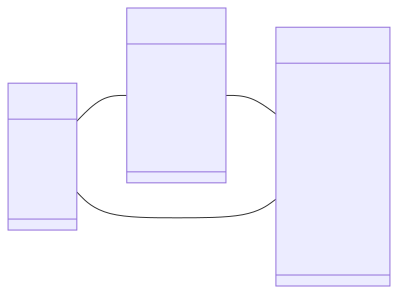
\includegraphics[scale=.8]{Illustrations/class_diagram.png}
	\caption{Klassendiagramm}
\end{figure}


% chapter datamodelling (end)


\chapter{Systemdesign} % (fold)
\label{sec:systemdesign}
Innerhalb dieses Abschnitts werden die konkret gewählten Technologien für die Entwicklung eines Systems beschrieben, das für Latentztests verwendet werden kann.
\section{Datenbankdesign} % (fold)
Für die Durchführung des Experiments wurden zwei Datenbanktypen verwendet, die nachfolgend mit ihrer spezifischen Konfiguration beschrieben werden.
\label{sec:datenbankdesign}
\subsection{Relationales Datenbankdesign} % (fold)
\label{sec:relationalesdatenbankdesign}

\begin{figure}[H]
	\centering
	\includegraphics[scale=0.6]{Illustrations/table_diagram.png}
	\caption{Datenbankdiagramm}
\end{figure}
\newpage
\noindent
Für die Erstellung einer relationale Datenbank aus dem gegebenen Datenmodell (Abb. 4.1) wurde dieses wie in Abb. 5.1 zu sehen angepasst, um die Beziehung zwischen \texttt{Person} und \texttt{Project} sowie \texttt{Person} und \texttt{Issue} abzubilden. Somit ergeben sich für die relationale Datenbank fünf Tabellen, die in einer PostgreSQL- Datenbank realisiert werden. Dabei wird PostgreSQL verwendet, weil es ein leistungsfähiges, objekt-relationales Open-Source-Datenbanksystem bietet. Die Datenbank wurde mit den in Abbildung 5.2 bis 5.6 beispielhaft dargestellten Beispieldaten befüllt, wobei 500 000 \texttt{Person}- sowie \texttt{Project}- und \texttt{Issue}-Objekte in die Datenbank eingefügt wurden. Durch die Verwendung von Zwischentabellen, wie \texttt{Person\_Issue} und \texttt{Person\_Project}, enthält die relationale Datenbank 2,5 Mio. Tupel mit einem Speicherbedarf von 215 MB. 

\begin{figure}[H]
	\centering
	\begin{tabular}{|l | l | l | l |}
	\hline
	pid & firstname & lastname & email \\
	\hline
	1 & Cecilla & Beningfield & cbeningfield9@wp.com \\
	\hline
	\end{tabular}
	\caption{Tupel der Tabelle ‚Person‘}
\end{figure}
\begin{figure}[H]
	\centering
	\begin{tabular}{|l | l |}
	\hline
	pid & iid \\
	\hline
	1 & 4894 \\
	\hline
	\end{tabular}
	\caption{Tupel der Tabelle ‚Person\_Issue‘}
\end{figure}
\begin{figure}[H]
	\centering
	\begin{tabular}{|l | l | l | l | l | l|}
	\hline
	iid & title & createdat & state & statereason & prid \\
	\hline
	1 & Dabfeed & 2023-06-10 00:00:00 & Open & Assigned & 586 \\
	\hline
	\end{tabular}
	\caption{Tupel der Tabelle ‚Issue‘}
\end{figure}
\begin{figure}[H]
	\centering
	\begin{tabular}{|l | l |}
	\hline
	pid & prid \\
	\hline
	1 & 714 \\
	\hline
	\end{tabular}
	\caption{Tupel der Tabelle ‚Person\_Project‘}
\end{figure}
\begin{figure}[H]
	\centering
	\begin{tabular}{|l | l | l |}
	\hline
	prid & title & createdat \\
	\hline
	1 & Asoka & 2022-02-17 00:00:00 \\
	\hline
	\end{tabular}
	\caption{Tupel der Tabelle ‚Project‘}
\end{figure}
\newpage


% subsection relationalesdatenbankdesign (end)
\subsection{Graphdatenbankdesign} % (fold)
\label{sec:graphsdatenbankdesign}
Die Erstellung einer Graphdatenbank erfordert keine definierten Tabellen, weil sie die Daten schemafrei speichert. Die Kanten werden bei der Erstellung entsprechend den Objekten benannt, was ebenso auf die Beziehungen zwischen den Knoten zutrifft. Als Graphdatenbank wurde auf Neo4j als eine der am weitesten verbreiteten Graphdatenbanken zurückgegriffen, die eine hohe Benutzerfreundlichkeit bietet. Abbildung 5.7 bietet eine Demonstration einer Beziehung zwischen jeweils einem Knoten. Die Kanten sind als gerichtete Kanten abgebildet, wobei \texttt{Person} zwei ausgehende Kanten, \texttt{Project} zwei eingehende und \texttt{Issue}jeweils sowohl eine eingehende als auch eine ausgehende Kante aufweist. Wie in der relationalen Datenbank wurden auch in der Graphdatenbank 500 000 Knoten pro Objekt erstellt. Hierbei waren jedoch keine Zwischentabellen zur Darstellung von Beziehungen nötig, wodurch in der Datenbank 1,5 Mio. Knoten vorliegen, die durch 2,01 Mio. Kanten verbunden sind. Hieraus ergibt sich eine Gesamtgröße von 197 MB.

\begin{figure}[H]
	\centering
	\includegraphics[scale=.8]{Illustrations/graph_diagram}
	\caption{Graphdiagramm}
\end{figure}
% subsection graphdatenbankdesign (end)

% section datenbankdesign (end)
\newpage
\section{Schnittstellendesign} % (fold)
\label{sec:schnittstellendesign}

\subsection{REST}
\label{sec:rest}
Bei REST wird für jedes Testszenario ein separater Endpunkt benötigt, wobei sechs Endpunkte mit unterschiedlicher Komplexität entworfen wurden.

\begin{itemize}
\item \colorbox{gray!20}{\textbf{HEAD api/resource}} wird verwendet, um einen Head-Request zur Bestimmung der Latenz der API durchzuführen..
\item Durch \colorbox{gray!20}{\textbf{GET api/issues?counter=x\&?joins=y}} kann die Menge der Ergebnistupel (x) und die Anzahl der auf der Datenbank durchgeführten Joins (y) bei der Anfrage bestimmt werden, wobei die in Abbildung 5.8 dargestellte Antwort erwartet wird.
\begin{figure}[H]
\begin{center}
\begin{BVerbatim}
   {
        "iid": 1,
        "title": "Pixope",
        "createdAt": "2024-07-23 00:00:00",
        "state": "Closed"
        "stateReason": "Cancelled"
    },
[...]
\end{BVerbatim}
\end{center}
\caption{‚GET api/issues?counter=x\&?joins=y‘-Response}
\end{figure}


\item \colorbox{gray!20}{\textbf{GET api/persons/:pid}}: Dieser Endpunkt ermöglicht das Abrufen einer bestimmten Person anhand ihrer ID, wobei die API ein JSON-Objekt zurückliefert, dass die \texttt{Person} mit den Attributen \texttt{Firstname, Lastname} und \texttt{E-Mail} beschreibt. (Abb. 5.9)
\begin{figure}[H]
\begin{center}
\begin{BVerbatim}
{
    "pid": 10,
    "firstname": "Cecilla",
    "lastname": "Beningfield",
    "email": "cbeningfield9@wp.com"
}
\end{BVerbatim}
\end{center}
\caption{‚GET api/persons/:pid‘-Response}
\end{figure}

\item Mit dem Endpunkt  \colorbox{gray!20}{\textbf{GET api/persons}} können alle in der Datenbank gespeicherten Person- Objekte abgerufen werden, wobei die Antwort 5000  \texttt{Project}-Objekte im JSON-Format umfasst. (Abb. 5.10)
\begin{figure}[H]
\begin{center}
\begin{BVerbatim}
[
    {
        "pid": 1,
        "firstname": "Ruby",
        "lastname": "Burchatt",
        "email": "rburchatt0@msn.com"
    },
	[...]
    {
        "pid": 5000,
        "firstname": "Murdoch",
        "lastname": "Simonitto",
        "email": "msimonittorr@google.ca"
    }
]
\end{BVerbatim}
\end{center}
\caption{‚GET api/persons‘-Response}
\end{figure}

\item Der Endpunkt \colorbox{gray!20}{\textbf{GET api/persons/:pid/projects/issue}} erhöht die Komplexität, weil hier nicht nur auf ein einzelnes Objekt zugegriffen wird. Stattdessen erfordert die Abfrage zur Bearbeitung mehrere Objekte, die miteinander in Abhängigkeit stehen. Die Antwort umfasst alle  \texttt{Issue}-Objekte, die in  \texttt{Project}-Objekten vorhanden sind, in denen eine  \texttt{Person} mitwirkt. (Abb. 5.11)
\begin{figure}[H]
\begin{center}
\begin{BVerbatim}
[
   {
        "iid": 1,
        "title": "Pixope",
        "createdAt": "2024-07-23 00:00:00",
        "state": "Closed"
        "stateReason": "Cancelled"
    },
    {
        "iid": 2876,
        "title": "Zoomlounge",
        "createdAt": "2020-08-26 00:00:00",
        "state": "Open"
        "stateReason": "Bug"
    },
]
\end{BVerbatim}
\end{center}
\caption{‚GET api/persons/:pid/projects/issue‘-Response}
\end{figure}

\item Der Endpunkt \colorbox{gray!20}{\textbf{POST api/persons/:pid/projects/:prid/issues}} ermöglicht das Erstellen eines neuen Issue in der Datenbank, um nicht nur Abfragen, sondern auch das Hinzufügen von Daten zu testen. Im Body der Anfrage wird ein  \texttt{Issue}-Objekt im JSON-Format übergeben. (Abb. 5.12)
\newline
\begin{figure}[H]
\begin{center}
\begin{BVerbatim}
{
    "title":"test",
    "createdAt":"2023-02-21T00:00:00",
    "state":"Open",
    "stateReason":"Bug"
}
\end{BVerbatim}
\end{center}
\caption{‚POST api/persons/:pid/projects/:prid/issues‘-Body}
\end{figure}
Die Antwort enthält das erstellte \texttt{Issue}, das eine gültige  \texttt{ID} sowie Verknüpfungen zu dem zugehörigen  \texttt{Project} und der  \texttt{Person} umfassen. (Abb. 5.13)
\begin{figure}[H]
\begin{center}
\begin{BVerbatim}
{
    "iid": 5207,
    "title": "test",
    "createdAt": "2023-02-21T00:00:00",
    "state": "Open",
    "stateReason": "Bug",
    "project": {
        "prid": 12,
        "title": "Y-find",
        "createdAt": "2021-01-10T00:00:00"
    },
    "assignee"{
        "pid": 1,
        "firstname": "Ruby",
        "lastname": "Burchatt",
        "email": "rburchatt0@msn.com"
    },
}
\end{BVerbatim}
\end{center}
\caption{‚POST api/persons/:pid/projects/:prid/issues‘-Response}
\end{figure}
\end{itemize}

% section rest (end)

\subsection{GraphQL}
Hinsichtlich der Art der Anfragen unterscheidet sich GraphQL stark von REST, denn es wird nur über den Endpunkt \colorbox{gray!20}{POST api/graphql}angesprochen, worüber sowohl Querys als auch Mutations abgedeckt werden. Die Anfragen werden im Body mithilfe der GraphQL-Query- Language definiert, die JSON ähnelt. Die in 5.2.1 definierten REST-Endpunkte wurden in GraphQL nachgebildet, sodass sie dieselbe Antwort liefern. Für einen HEAD-Request bietet GraphQL nativ jedoch keine Lösung, weshalb in GraphQL APIs der HEAD-Request identisch wie in den REST-APIs implementiert wurde. Der parametrisierte Endpunkt aus der REST-API wurde in GraphQL entsprechend der Darstellung in Abb. 5.14 umgesetzt, wobei bei \texttt{Counter} Werte zwischen 0 und 1,5 Mio sowie bei  \texttt{Joins} Werte zwischen 0 und 3 möglich sind.

\begin{figure}[H]
\begin{center}
\begin{BVerbatim}
query{
    issuesCount(counter: 10, joins: 1){
	iid
	title 
	createdAt 
	state 
	stateReason
    }
}
\end{BVerbatim}
\end{center}
\caption{GraphQ-Query GET api/issues?counter=x\&?joins=y}
\end{figure}
\noindent
Die in Abbildung 5.15 dargestellte Query ist dem REST-Endpunk \colorbox{gray!20}{GET api/persons/:pid} äquivalent, wobei ebenfalls eine ID übergeben wird. Allerdings können die in der Antwort enthaltenen Felder explizit gewählt werden. In diesem Beispiel wurden \texttt{PID},  \texttt{Firstname},  \texttt{Lastname} sowie die  \texttt{E-Mail} genutzt, um dieselbe Antwort wie beim REST-Endpunkt zu erhalten.
\begin{figure}[H]
\begin{center}
\begin{BVerbatim}
query{
    person(id : 10){
	pid
	firstname
	lastname
	email
    }
}
\end{BVerbatim}
\end{center}
\caption{GraphQL-Query-Äquivalent zu GET api/persons/:pid}
\end{figure}
\noindent
Der REST-Endpunkt \colorbox{gray!20}{GET api/persons} wird von der GraphQL-Query in Abbildung 5.16 repräsentiert, wobei dieselben Felder wie in der vorherigen Abfrage selektiert werden. Jedoch wird hierbei die Query \colorbox{gray!20}{persons} angesprochen, wodurch alle  \texttt{Person} Objekte der Datenbank abgerufen werden.
\begin{figure}[H]
\begin{center}
\begin{BVerbatim}
query {
    persons {
        pid
        firstname
        lastname
        email
    }
}
\end{BVerbatim}
\end{center}
\caption{GraphQL-Query-Äquivalent zu GET api/persons}
\end{figure}
\noindent
Abbildung 5.17 zeigt die GraphQL-Query, die dem REST-Endpunkt \colorbox{gray!20}{GET api/persons/} \colorbox{gray!20}{:pid/projects/issue} entspricht. Hierbei werden die im Schema definierten Querys geschachtelt, um eine Abfrage zu erhalten, die die Abhängigkeiten zwischen den Objekten repräsentiert.
\begin{figure}[H]
\begin{center}
\begin{BVerbatim}
query{
    person(id : 10){
        projects{
	    issues{
		iid
		title
		createdAt
		state
		stateReason
	    }
        }
    }
}
\end{BVerbatim}
\end{center}
\caption{GraphQL-Query-Äquivalent zu GET api/persons/:pid/projects/issue}
\end{figure}
\noindent
Um den REST-Endpunkt \colorbox{gray!20}{POST api/persons/:pid/projects/:prid/issues} nachzubilden wurde die in Abb. 5.18 dargestellte Mutation entwickelt. Hierbei wird ein Input-Objekt definiert, das die zur Erstellung des Issue benötigten Attribute beinhaltet. Danach kann selektiert werden, welche Felder in der Antwort enthalten sind.
\begin{figure}[H]
\begin{center}
\begin{BVerbatim}
mutation{
    createIssue(input:{
	title : „Bug in Login“
	createdAt : „2024-12-03T12:30:00
	state : „Open“
	stateReason : „Error in Login“
	prid: 80
	pid: 10
	}){
	iid
	title
	state
	stateReason
	createdAt
    }
}
\end{BVerbatim}
\end{center}
\caption{GraphQL-Query-Äquivalent zu POST api/persons/:pid/projects/:prid/issues}
\end{figure}

\label{sec:graphql}
% section graphql (end)

% section schnittstellendesign (end)
\section{Testumgebung} % (fold)
\label{sec:testumgebung}
Zur Ermittlung der Latenzzeiten wurden API-Abfragen durchgeführt, wobei die Antwortzeiten in Millisekunden protokolliert wurden. Dafür wurde eine Testumgebung mit zwei unterschiedlichen Endgeräten benötigt, um die Last auf mehrere Geräte zu verteilen. Die APIs liefen auf einem Server in Frankfurt, der mit vier Kernen, 24 GB Arbeitsspeicher, einer 1 Gbit-Internetverbindung und Ubuntu 22.04 als Betriebssystem ausgestattet ist.
\newline
Die Abfragen erfolgten von einem PC mit acht Kernen, 32 GB Arbeitsspeicher, einer 50 Mbit- Internetverbindung und Windows 10 als Betriebssystem, wobei die durchschnittliche Latenz (Ping) zwischen Server und PC 24 ms betrug. Weil ein Ping jedoch nur auf ISO-Schicht 3 agierte, wurde vor jedem Testdurchlauf mithilfe von HEAD-Requests, die in Kapitel 5.2.1 beschrieben wurden, eine Latenz zwischen den Endgeräten ermittelt, die alle ISO-Schichten durchlief. Um Schwankungen bei der Netzwerkauslastung und der Systembelastung zu minimieren, wurden pro Testszenario und API jeweils hundert Anfragen ausgeführt. Insgesamt ergibt dies bei vier APIs und 25 Testszenarien eine Datengrundlage von 10 000 Latenzzeiten.


% section testumgebung (end)


% chapter Systemdesign (end)
\chapter{Implementierung} % (fold)
\label{sec:implementierung}
Nachfolgend soll die Implementierung der verschiedenen APIs, sowie die Grundprinzipien während der Implementierung, beschrieben werden. Der Source Code der Implementierung ist unter MIT Lizenz auf GitHub veröffentlicht. \citep{me}
\section{Grundprinzipien während der Implementierung} % (fold)
\label{sec:prinzipien}
Im Rahmen der Implementierung dieser Anwendung wurden verschiedene Grundprinzipien beachtet, die sowohl die Qualität als auch die Erweiterbarkeit der Anwendungen  sicherstellen. Die Wahl der verwendeten Technologien sowie die Anwendung bewährter Praktiken standen dabei im Vordergrund. Als Basis für die Entwicklung wurde Java JDK 17.0.10 Corretto gewählt, da diese Version eine Long-Term-Support (LTS)-Version darstellt und damit eine stabile und sichere Grundlage für die Entwicklung bietet. Amazon Corretto bietet eine optimierte JVM, wodurch alle Softwarebestandteile auf jeder Plattform mit einer zertifizierten JAVA Virtual Machine lauffähig sind. Ergänzt wurde das JDK durch Spring Boot Version 3.3.4, eine weit verbreitete Plattform für die Entwicklung von Webanwendungen und Microservices. Spring Boot ermöglicht eine schnelle und einfache Konfiguration von Anwendungen und vereinfacht den Entwicklungsprozess durch das Automatisieren von häufig auftretenden Aufgaben, wie etwa der Konfiguration von Servern und Datenbankverbindungen.
\noindent
Ein zentrales Konzept während der Implementierung war die Verwendung von Dependency Injection. Diese Technik sorgt dafür, dass die Abhängigkeiten zwischen den einzelnen Komponenten der Anwendung nicht hart kodiert sind, sondern zur Laufzeit durch den DI-Container von Spring injiziert werden. DI fördert die Entkopplung von Komponenten, was zu einer besseren Testbarkeit, Flexibilität und Wartbarkeit des Codes führt. Da der Code durch DI in unabhängige, gut getestete Module unterteilt wird, lässt er sich leicht erweitern und an geänderte Anforderungen anpassen. Zudem trägt DI zur Verbesserung der Lesbarkeit des Codes bei, da Abhängigkeiten nicht explizit an anderen Stellen erstellt werden müssen.
\noindent
Die Implementierung der Anwendung erfolgte unter der Berücksichtigung von Best Practices, die die Qualität des Codes sicherstellen und eine effiziente, langfristige Wartung ermöglichen. Ein wesentlicher Aspekt war hierbei die Modularität der Lösung. Die Anwendung wurde so strukturiert, dass jede Komponente eine klare, abgegrenzte Verantwortung übernimmt. Dies sorgt nicht nur für eine bessere Nachvollziehbarkeit des Codes, sondern erleichtert auch das Testen und die Erweiterung von Funktionalitäten. Bestehende Komponenten können so problemlos durch neue ersetzt oder erweitert werden, ohne die gesamte Anwendung zu beeinträchtigen.




% section prinzipien (end)

\section{Post REST} % (fold)
\label{sec:postrest}
In dieser Arbeit steht "PostREST" für die PostgreSQL REST-API, die eine Schnittstelle für den Zugriff auf eine PostgreSQL-Datenbank über HTTP-Anfragen bietet. Diese API implementiert eine Reihe von Endpunkten, die in Abschnitt 5.2.1 der Arbeit definiert sind. Diese Endpunkte sind dafür verantwortlich, bestimmte Anfragen zu bearbeiten und entsprechende Antworten zurückzugeben.
\noindent
Die zentrale Komponente, die dafür sorgt, dass die Endpunkte korrekt verarbeitet werden, ist die Controller-Klasse(vgl Abb. 6.1). In dieser Klasse sind die Endpunkte integriert, wobei jeder Endpunkt mit seinen spezifischen Pfadvariablen und den Rückgabewerten versehen ist. Die Controller-Klasse übernimmt die Aufgabe, die richtigen Methoden auszuführen, wenn eine Anfrage an einen bestimmten Endpunkt gestellt wird.
\noindent
Der PostrestController ist die konkrete Implementierung des Controllers, der die Geschäftslogik verarbeitet. Er ruft den DBService auf, welcher das Interface IDBService implementiert. Das Interface definiert die Methoden, die notwendig sind, um Daten aus den zugrunde liegenden Datenbanken abzurufen. Diese Methoden kapseln die Logik für den Datenbankzugriff und sind so gestaltet, dass sie von der Controller-Klasse verwendet werden können, um die richtigen Informationen zu erhalten.
\noindent
Die Kommunikation zwischen den verschiedenen Schichten der Anwendung erfolgt durch Dependency Injection. Das bedeutet, dass die verschiedenen Komponenten nicht direkt in der Controller-Klasse erzeugt werden, sondern von außen in die Klasse injiziert werden. In diesem Fall werden die Repositorys der verschiedenen Entitäten in die Controller-Klasse injiziert. Diese Repositorys sind verantwortlich für den direkten Datenbankzugriff und beinhalten die notwendigen Methoden und SQL-Abfragen, die zum Abrufen und Verwalten der Daten in der Datenbank erforderlich sind.
\noindent
Nachdem die Daten erfolgreich aus der Datenbank abgefragt wurden, werden sie durch die Hierarchie der Anwendung weitergegeben. Der PostrestController sorgt dafür, dass die abgerufenen Daten in das gewünschte Format für die API-Antwort umgewandelt werden. Dies ist in diesem Fall das JSON-Format, dass dann dem Nutzer der API als Antwort übermittelt wird. Diese Antwort enthält die angeforderten Informationen, die der Nutzer über die API abgefragt hat.
\begin{figure}[H]
	\centering
	\includegraphics[scale=0.5]{Illustrations/postrest.png}
	\caption{Java Klassen PostREST}
\end{figure}
% section postrest (end)

\section{Post Graph} % (fold)
\label{sec:postgraph}
Hierbei handelt es sich um eine GraphQL-API, die mit einer PostgreSQL-Datenbank verbunden ist. Das Schema, das die Arbeitsweise der API beschreibt, wird – wie bei GraphQL üblich – in der Datei schema.graphqls definiert. In dieser Datei sind die verschiedenen Datentypen sowie die möglichen Queries und Mutationen beschrieben, die zur Abfrage und Bearbeitung der Daten verwendet werden können. 
\noindent
In den folgenden Abbildungen sind Beispiele für einen Typ, verschiedene Queries und eine Mutation dargestellt, wie sie in der schema.graphqls-Datei definiert sind:
\begin{figure}[H]
\begin{center}
\begin{BVerbatim}
type Issue{
    iid : ID!
    title : String
    createdAt : String
    state : String
    stateReason : String
}
\end{BVerbatim}
\end{center}
\caption{Type aus der Schema.graphqls}
\end{figure}
\begin{figure}[H]
\begin{center}
\begin{BVerbatim}
type Query{
    persons: [Person]
    person(id:ID!): Person
    projects: [Project]
    project(id:ID!) : Project
    issues : [Issue]
    issue(id: String): Issue
}
\end{BVerbatim}
\end{center}
\caption{Queries aus der Schema.graphqls}
\end{figure}
\begin{figure}[H]
\begin{center}
\begin{BVerbatim}

type Mutation {
    createIssue(input: IssueInput): Issue
}
\end{BVerbatim}
\end{center}
\caption{Mutation aus der Schema.graphqls}
\end{figure}
\newpage
\noindent
Die zentrale Komponente für die Verarbeitung von Anfragen ist die Java-Klasse Query(vgl. Abb. 6.5). In dieser Klasse werden Methoden implementiert, die die Bearbeitung der Anfragen gemäß den Strukturen in der schema.graphqls-Datei ermöglichen. Diese Methoden greifen auf die Repositories der Modelklassen zu, um Datenbankoperationen durchzuführen. Die Repositories enthalten die erforderlichen Methoden und Logiken, um Daten in der PostgreSQL-Datenbank zu lesen oder zu ändern.
\noindent
Ein hervorstechendes Merkmal von GraphQL ist der Einsatz von Resolvern. Diese kommen zum Einsatz, um Felder zu verarbeiten, die auf Daten aus anderen Quellen oder Datenbanken basieren. Resolver stellen sicher, dass die relevanten Daten korrekt abgerufen und in der gewünschten Struktur zurückgegeben werden.
\noindent
Die Repositories werden in die benötigten Klassen injiziert, sodass sie nicht direkt innerhalb der Anwendung erstellt werden müssen.
\noindent
Nach erfolgreicher Bearbeitung einer Anfrage liefert die GraphQL-API die Daten im vorgegebenen GraphQL-Format an den Nutzer zurück. Dies gewährleistet eine flexible und leistungsfähige Schnittstelle zur Abfrage und Manipulation der Daten in der zugrunde liegenden PostgreSQL-Datenbank.
\begin{figure}[H]
	\centering
	\includegraphics[scale=0.5]{Illustrations/postgraph.png}
	\caption{Java Klassen PostGraph}
\end{figure}
% section postgraph (end)

\section{Neo4REST} % (fold)
\label{sec:neo4rest}
Neo4REST ist eine REST-API, die den Zugriff auf eine Neo4j-Datenbank ermöglicht. Analog zur Struktur von PostREST bietet Neo4REST eine Reihe von Endpunkten, die zur Bearbeitung spezifischer Anfragen und zur Rückgabe der entsprechenden Antworten dienen. Die Details dieser Endpunkte sind in Abschnitt 5.2.2 definiert.
\noindent 
Die Verarbeitung der Endpunkte wird durch die zentrale Controller-Klasse sichergestellt (vgl. Abb. 6.7). Wie bei PostREST sind hier die spezifischen Pfadvariablen, Parameter und Rückgabewerte der Endpunkte definiert. Die Controller-Klasse sorgt dafür, dass die passenden Methoden aufgerufen werden, sobald eine Anfrage an einen der Endpunkte gestellt wird.
\noindent 
Der Neo4RestController übernimmt dabei die Geschäftslogik und delegiert datenbankbezogene Aufgaben an den DBService, der das Interface IDBService implementiert. Dieses Interface definiert die für den Zugriff auf die Neo4j-Datenbank erforderlichen Methoden. Die Umsetzung der konkreten Abfragen erfolgt über Repositories, die für die Durchführung der Cypher-Abfragen zuständig sind. Diese Repositorys abstrahieren den Datenbankzugriff und bieten wiederverwendbare Methoden, um auf die in Neo4j gespeicherten Daten zuzugreifen oder sie zu ändern.
\noindent 
Die in der Datenbank abgefragten Informationen werden, wie auch bei PostREST, durch die Schichten der Anwendung weitergeleitet und im Controller in das JSON-Format umgewandelt, bevor sie als API-Antwort zurückgegeben werden. So stellt Neo4REST sicher, dass der Nutzer die angeforderten Informationen oder den Status einer Operation im passenden Format erhält.
\begin{figure}[H]
	\centering
	\includegraphics[scale=0.5]{Illustrations/neo4rest.png}
	\caption{Java Klassen Neo4REST}
\end{figure}
% section neo4rest (end)

\section{Neo4Graph} % (fold)
\label{sec:neo4graph}
Die Neo4Graph-API ist eine GraphQL-API, die mit einer Neo4j-Datenbank verbunden ist. Das Schema, das bereits in der PostGraph-API beschrieben wurde, wird auch in Neo4Graph auf ähnliche Weise implementiert. Wie bei PostGraph kommen auch hier Cypher-Abfragen zum Einsatz, um mit der Neo4j-Datenbank zu interagieren. Die Methoden nutzen die Neo4j-Clientbibliothek, um Knoten und Kanten effizient zu durchsuchen und Datenbankoperationen durchzuführen.
\noindent
Ein weiteres gemeinsames Merkmal beider APIs ist der Einsatz von Resolvern. In Neo4Graph werden diese ebenfalls verwendet, um Felder zu bearbeiten, die auf Beziehungen oder aggregierten Daten im Graphen basieren. Resolver sorgen dafür, dass die benötigten Daten korrekt abgerufen und in der gewünschten Struktur zurückgegeben werden.
\noindent
Nach der Bearbeitung einer Anfrage liefert die GraphQL-API die Daten im standardisierten GraphQL-Format an den Nutzer, was eine konsistente und leistungsfähige Schnittstelle zur Abfrage und Bearbeitung der Daten in der Neo4j-Datenbank sicherstellt

\begin{figure}[H]
	\centering
	\includegraphics[scale=0.5]{Illustrations/neo4graph.png}
	\caption{Java Klassen Neo4Graph}
\end{figure}
% section neo4graph (end)
\section{API-Response Test} % (fold)
\label{sec:test}
Eine Anwendung wurde entwickelt, um API-Anfragen von einem entfernten System durchzuführen. Diese Anwendung enthält für jeden Endpunkt eine Methode(vgl. Abb. 6.8), die jeweils 100 Abfragen in einer Schleife ausführt. Falls für eine Abfrage eine ID erforderlich ist, wird diese mithilfe der Klasse Random aus java.util.Random generiert. Die Abfragen für den parametrisierten Endpunkt werden mit den Joins von 0 bis 3 und den Ergebnistupeln 1, 100, 1000, 10.000 und 100.000 durchgeführt. Die Abfragezeit wird ermittelt, indem die aktuelle Systemzeit in Millisekunden unmittelbar vor der Ausführung der Abfrage erfasst und von der Zeit nach Abschluss der Abfrage abgezogen wird.
\begin{figure}[H]
	\centering
	\includegraphics[scale=0.5]{Illustrations/apiresponsetest.png}
	\caption{Java Klassen Neo4Graph}
\end{figure}
% section test (end)
% chapter implementierung (end)
\chapter{Ergebnisse} % (fold)
\label{sec:ergebnisse}
Im Nachfolgenden werden die Ergebnisse der Latenztests der oben eingeführten APIs dargestellt.

\noindent
Wie in Abbildung 7.1 zusehen ist, hat die PostgreSQL REST-API eine höhere Latenzzeit als die GraphQL PostgeSQL. Dies deutet darauf hin, dass die GraphQL API bei der Abfrage eines spezifischen Personenobjekts, anhand der Personen-ID in kombination mit einer relationalen Datenbank effizientere Abfragen und eine bessere Performance bei der Verarbeitung bietet. Ähnliches zeigt sich bei einer Neo4j Datenbank. Auch hier hat die Neo4j GraphQL API niedrigere Latenzzeiten als die REST-API. Allerdings sind die Latenzen bei Neo4j minimal höher als bei dem realtionalen Pendant. Das deutet darauf hin, dass Postgres bei dieser Anfrage eine performantere Verarbeitung von Abfragen ermöglicht. Zusammenfassend kann man für diese Anfrage sagen, dass GraphQL sowohl in kombination mit einer relationalen, als auch einer Graphdatenbank eine niedrigere Latenz aufweist. Zudem ist Postgres bei dieser Anfrage insgesamt ein wenig performanter als neo4j.
\newline
In Abbildung 7.2 sind die Latenzen für die komplexere Anfrge, die alle Personenobjekte aus der Datenbank zurückliefert dargestellt. Bei den APIs die mit Postgres implementiert sind ist eine deutlich niedrigere Latenz zu sehen, als bei den mit neo4j implementierten. GraphQL hat hierbei sowohl bei der relationalen Datenbank als auch bei der Graphdatenbank im Median eine niedrigere Latenz. REST ist somit in beiden Fällen die unperformantere API.
\newline
Wenn nun die Anfragekomplexität steigt, wodurch sich die Abhängigkeit zwischen den Objekten in der Datenbank erhöht, ist deutlich zu sehen, dass die Streuung bei der Postgres REST-API höher ist als bei allen anderen APIs (vgl Abb.7.3). Zudem ist diese API diejenige mit der höchsten Latenz. Allerdings liegt die Neo4j REST-API im Median über den Postgres REST-API. Beide GraphQL APIs weißen erneut eine deutlich niedrigere Latenz auf.
\newline
Bei der Speicherung in eine Datenbank ist ein deutlich anderes Bild zu sehen. Wie in Abbildung 7.4 zusehen, ist hierbei die Postgres REST-API diejenige mit der geringsten LAtenz. Dicht gefolgt von der Postgres GraphQL API. Eine deutlich höhere Latenz ist bei den neo4j APIs zu erkennen. Hierbei ist allerdings die GraphQL API die performantere.




\begin{figure}[htbp]
 \centering
	\begin{tikzpicture}
	    \begin{axis}[
	        boxplot/draw direction=y, 
	        xlabel={API}, 
	        ylabel={ms}, 
	        xtick={1,2,3,4}, 
	        xticklabels={Post Rest, Post Graph, Neo4 Rest, Neo4 Graph}, 
	        ymin=50, ymax=65,
	       ytick distance=1,
                  width=15cm,
	       height= 18cm
	    ]
	       \addplot+[
	            boxplot prepared={
	                median=52,
	                upper quartile=55,
	                lower quartile=52, 
	                upper whisker=59,
	                lower whisker=51
	            },
	            draw=black
	        ] coordinates {};
	        \addplot+[
	            boxplot prepared={
	                median=53,
	                upper quartile=53,
	                lower quartile=53, 
	                upper whisker=54,
	                lower whisker=52
	            },
	            draw=black
	        ] coordinates {};
	         \addplot+[
	            boxplot prepared={
	                median=52,
	                upper quartile=58,
	                lower quartile=52, 
	                upper whisker=63,
	                lower whisker=51
	            },
	            draw=black
	        ] coordinates {};
	       \addplot+[
	            boxplot prepared={
	                median=52,
	                upper quartile=53,
	                lower quartile=52, 
	                upper whisker=54,
	                lower whisker=51
	            },
	            draw=black
	        ] coordinates {};
	    \end{axis}
	\end{tikzpicture}
\caption{HEAD /api/resource}
\end{figure}




\begin{figure}
\centering
\begin{tikzpicture}[scale=1.9]
\begin{axis}[
    axis lines = middle,
    xlabel = {x},
    ylabel = {y},
    zlabel = {z},
    xmode = log,
    width=10cm,
    height=10cm,
    grid = major,
    enlarge x limits = true,
    view={0}{0},
    ymin=0, ymax=3,  
]
% Linie und Punkte für die ersten Punkte (rot)
\addplot3+[
    only marks, 
    mark=*,
    red,
    mark options={fill=red} % Innere des Punktes rot färben
] coordinates {
    (1, 0, 111)
    (100, 0, 121)
    (1000, 0, 135)
    (10000, 0, 272)
    (100000, 0, 426.5)
};
\addplot3[
    red, % Linie durch die Punkte
    mark=none % keine Markierungen an der Linie
] coordinates {
    (1, 0, 111)
    (100, 0, 121)
    (1000, 0, 135)
    (10000, 0, 272)
    (100000, 0, 426.5)
};
% Linie und Punkte für die zweiten Punkte (blau)
\addplot3+[
    only marks, 
    mark=square*,
    blue,
    mark options={fill=blue} % Innere des Punktes blau färben
] coordinates {
    (1, 1, 111)
    (100, 1, 122)
    (1000, 1, 134)
    (10000, 1, 271.5)
    (100000, 1, 468)
};
\addplot3[
    blue, % Linie durch die Punkte
    mark=none % keine Markierungen an der Linie
] coordinates {
    (1, 1, 111)
    (100, 1, 122)
    (1000, 1, 134)
    (10000, 1, 271.5)
    (100000, 1, 468)
};
% Linie und Punkte für die vierten Punkte (orange)
\addplot3+[
    only marks, 
    mark=diamond*,
    orange,
    mark options={fill=orange} % Innere des Punktes orange färben
] coordinates {
    (1, 3, 111)
    (100, 3, 119.5)
    (1000, 3, 146)
    (10000, 3, 267)
    (100000, 3, 492.5)
};
\addplot3[
    orange, % Linie durch die Punkte
    mark=none % keine Markierungen an der Linie
] coordinates {
    (1, 3, 111)
    (100, 3, 119.5)
    (1000, 3, 146)
    (10000, 3, 267)
    (100000, 3, 492.5)
};
\end{axis}
\end{tikzpicture}
\caption{PostREST parametriesierte Abfragen}
\end{figure}

\begin{figure}
\centering
\begin{tikzpicture}[scale=1.9]
\begin{axis}[
    axis lines = middle,
    xlabel = {x},
    ylabel = {y},
    zlabel = {z},
    xmode = log,
    width=10cm,
    height=10cm,
    grid = major,
    enlarge x limits = true,
    view={0}{0},
    ymin=0, ymax=3,  
]
% Linie und Punkte für die ersten Punkte (rot)
\addplot3+[
    only marks, 
    mark=*,
    red,
    mark options={fill=red} % Innere des Punktes rot färben
] coordinates {
    (1, 0, 56)
    (100, 0, 66)
    (1000, 0, 87.5)
    (10000, 0, 240.5)
    (100000, 0, 1815.5)
};
\addplot3[
    red, % Linie durch die Punkte
    mark=none % keine Markierungen an der Linie
] coordinates {
    (1, 0, 56)
    (100, 0, 66)
    (1000, 0, 87.5)
    (10000, 0, 240.5)
    (100000, 0, 1815.5)
};
% Linie und Punkte für die zweiten Punkte (blau)
\addplot3+[
    only marks, 
    mark=square*,
    blue,
    mark options={fill=blue} % Innere des Punktes blau färben
] coordinates {
    (1, 1, 94)
    (100, 1, 103)
    (1000, 1, 129)
    (10000, 1, 283.5)
    (100000, 1, 1831.5)
};
\addplot3[
    blue, % Linie durch die Punkte
    mark=none % keine Markierungen an der Linie
] coordinates {
    (1, 1, 94)
    (100, 1, 103)
    (1000, 1, 129)
    (10000, 1, 283.5)
    (100000, 1, 1831.5)
};
% Linie und Punkte für die vierten Punkte (orange)
\addplot3+[
    only marks, 
    mark=diamond*,
    orange,
    mark options={fill=orange} % Innere des Punktes orange färben
] coordinates {
    (1, 3, 55)
    (100, 3, 65)
    (1000, 3, 91.5)
    (10000, 3, 292)
    (100000, 3, 1792.5)
};
\addplot3[
    orange, % Linie durch die Punkte
    mark=none % keine Markierungen an der Linie
] coordinates {
    (1, 3, 55)
    (100, 3, 65)
    (1000, 3, 91.5)
    (10000, 3, 292)
    (100000, 3, 1792.5)
};
\end{axis}
\end{tikzpicture}
\caption{PostGraph parametriesierte Abfragen}
\end{figure}



\begin{figure}
\centering
\begin{tikzpicture}[scale=1.9]
\begin{axis}[
    axis lines = middle,
    xlabel = {x},
    ylabel = {y},
    zlabel = {z},
    xmode = log,
    width=10cm,
    height=10cm,
    grid = major,
    enlarge x limits = true,
    view={0}{0},
    ymin=0, ymax=3,  
]
% Linie und Punkte für die ersten Punkte (rot)
\addplot3+[
    only marks, 
    mark=*,
    red,
    mark options={fill=red} % Innere des Punktes rot färben
] coordinates {
    (1, 0, 119)
    (100, 0, 126)
    (1000, 0, 147)
    (10000, 0, 282)
    (100000, 0, 1673)
};
\addplot3[
    red, % Linie durch die Punkte
    mark=none % keine Markierungen an der Linie
] coordinates {
    (1, 0, 119)
    (100, 0, 126)
    (1000, 0, 147)
    (10000, 0, 282)
    (100000, 0,1673)
};
% Linie und Punkte für die zweiten Punkte (blau)
\addplot3+[
    only marks, 
    mark=square*,
    blue,
    mark options={fill=blue} % Innere des Punktes blau färben
] coordinates {
    (1, 1, 113.5)
    (100, 1, 124)
    (1000, 1, 143.5)
    (10000, 1, 269)
    (100000, 1, 1466)
};
\addplot3[
    blue, % Linie durch die Punkte
    mark=none % keine Markierungen an der Linie
] coordinates {
    (1, 1, 113.5)
    (100, 1, 124)
    (1000, 1, 143.5)
    (10000, 1, 269)
    (100000, 1, 1466)
};
% Linie und Punkte für die vierten Punkte (orange)
\addplot3+[
    only marks, 
    mark=diamond*,
    orange,
    mark options={fill=orange} % Innere des Punktes orange färben
] coordinates {
    (1, 3, 112)
    (100, 3, 122)
    (1000, 3, 145)
    (10000, 3, 269)
    (100000, 3, 1371)
};
\addplot3[
    orange, % Linie durch die Punkte
    mark=none % keine Markierungen an der Linie
] coordinates {
    (1, 3, 112)
    (100, 3, 122)
    (1000, 3, 145)
    (10000, 3, 269)
    (100000, 3, 1371)
};
\end{axis}
\end{tikzpicture}
\caption{Neo4REST parametriesierte Abfragen}
\end{figure}


\begin{figure}
\centering
\begin{tikzpicture}[scale=1.9]
\begin{axis}[
    axis lines = middle,
    xlabel = {x},
    ylabel = {y},
    zlabel = {z},
    xmode = log,
    width=10cm,
    height=10cm,
    grid = major,
    enlarge x limits = true,
    view={0}{0},
    ymin=0, ymax=3,  
]
% Linie und Punkte für die ersten Punkte (rot)
\addplot3+[
    only marks, 
    mark=*,
    red,
    mark options={fill=red} % Innere des Punktes rot färben
] coordinates {
    (1, 0, 58)
    (100, 0, 70)
    (1000, 0, 105.5)
    (10000, 0, 391)
    (100000, 0, 2726.5)
};
\addplot3[
    red, % Linie durch die Punkte
    mark=none % keine Markierungen an der Linie
] coordinates {
    (1, 0, 58)
    (100, 0, 70)
    (1000, 0, 105.5)
    (10000, 0, 391)
    (100000, 0,2726.5)
};
% Linie und Punkte für die zweiten Punkte (blau)
\addplot3+[
    only marks, 
    mark=square*,
    blue,
    mark options={fill=blue} % Innere des Punktes blau färben
] coordinates {
    (1, 1, 59)
    (100, 1, 70)
    (1000, 1, 102.5)
    (10000, 1, 330)
    (100000, 1, 2484.5)
};
\addplot3[
    blue, % Linie durch die Punkte
    mark=none % keine Markierungen an der Linie
] coordinates {
    (1, 1, 59)
    (100, 1, 70)
    (1000, 1, 102.5)
    (10000, 1, 330)
    (100000, 1, 2484.5)
};
% Linie und Punkte für die vierten Punkte (orange)
\addplot3+[
    only marks, 
    mark=diamond*,
    orange,
    mark options={fill=orange} % Innere des Punktes orange färben
] coordinates {
    (1, 3, 57)
    (100, 3, 69)
    (1000, 3, 96)
    (10000, 3, 317)
    (100000, 3, 2396.5)
};
\addplot3[
    orange, % Linie durch die Punkte
    mark=none % keine Markierungen an der Linie
] coordinates {
    (1, 3, 57)
    (100, 3, 69)
    (1000, 3, 96)
    (10000, 3, 317)
    (100000, 3, 2396.5)
};
\end{axis}
\end{tikzpicture}
\caption{Neo4Graph parametriesierte Abfragen}
\end{figure}















\begin{figure}[htbp]
 \centering
	\begin{tikzpicture}
	    \begin{axis}[
	        boxplot/draw direction=y, 
	        xlabel={API}, 
	        ylabel={ms}, 
	        ytick distance=5,
	        xtick={1,2,3,4}, 
	        xticklabels={Post Rest, Post Graph, Neo4 Rest, Neo4 Graph}, 
	        ymin=50, ymax=150,
		width=15cm,
		height= 18cm
	    ]
	        \addplot+[
	            boxplot prepared={
	                median=109,
	                upper quartile=110,
	                lower quartile=108, 
	                upper whisker=113,
	                lower whisker=107
	            },
	            draw=black
	        ] coordinates {};
	        \addplot+[
	            boxplot prepared={
	                median=56,
	                upper quartile=58,
	                lower quartile=56, 
	                upper whisker=60,
	                lower whisker=54
	            },
	            draw=black
	        ] coordinates {};
	        \addplot+[
	            boxplot prepared={
	                median=113,
	                upper quartile=115,
	                lower quartile=111, 
	                upper whisker=119,
	                lower whisker=110
	            },
	            draw=black
	        ] coordinates {};
	       \addplot+[
	            boxplot prepared={
	                median=58,
	                upper quartile=59,
	                lower quartile=57, 
	                upper whisker=62,
	                lower whisker=56
	            },
	            draw=black
	        ] coordinates {};
	    \end{axis}
	\end{tikzpicture}
\caption{GET /api/persons/:pid}
\end{figure}

\begin{figure}[htbp]
 \centering
	\begin{tikzpicture}
	    \begin{axis}[
	        boxplot/draw direction=y, 
	        xlabel={API}, 
	        ylabel={ms}, 
	        xtick={1,2,3,4}, 
	        xticklabels={Post Rest, Post Graph, Neo4 Rest, Neo4 Graph}, 
	        ymin=50, ymax=590,
                  ytick distance=20,
                  width=15cm,
	       height= 18cm
	    ]
	        \addplot+[
	            boxplot prepared={
	                median=264,
	                upper quartile=274,
	                lower quartile=259, 
	                upper whisker=293,
	                lower whisker=237
	            },
	            draw=black
	        ] coordinates {};
	        \addplot+[
	            boxplot prepared={
	                median=206,
	                upper quartile=214,
	                lower quartile=198, 
	                upper whisker=233,
	                lower whisker=178
	            },
	            draw=black
	        ] coordinates {};
	         \addplot+[
	            boxplot prepared={
	                median=539,
	                upper quartile=551,
	                lower quartile=529, 
	                upper whisker=579,
	                lower whisker=499
	            },
	            draw=black
	        ] coordinates {};
	       \addplot+[
	            boxplot prepared={
	                median=499,
	                upper quartile=509,
	                lower quartile=494, 
	                upper whisker=531,
	                lower whisker=482
	            },
	            draw=black
	        ] coordinates {};
	    \end{axis}
	\end{tikzpicture}
\caption{GET /api/persons}
\end{figure}

\begin{figure}[htbp]
 \centering
	\begin{tikzpicture}
	    \begin{axis}[
	        boxplot/draw direction=y, 
	        xlabel={API}, 
	        ylabel={ms}, 
	        xtick={1,2,3,4}, 
	        xticklabels={Post Rest, Post Graph, Neo4 Rest, Neo4 Graph}, 
	        ymin=50, ymax=140,
	        ytick distance=5,
                  width=15cm,
	       height= 18cm
	    ]
	        \addplot+[
	            boxplot prepared={
	                median=111,
	                upper quartile=119,
	                lower quartile=109, 
	                upper whisker=134,
	                lower whisker=107
	            },
	            draw=black
	        ] coordinates {};
	        \addplot+[
	            boxplot prepared={
	                median=56,
	                upper quartile=57,
	                lower quartile=56, 
	                upper whisker=58,
	                lower whisker=55
	            },
	            draw=black
	        ] coordinates {};
	         \addplot+[
	            boxplot prepared={
	                median=115,
	                upper quartile=117,
	                lower quartile=113, 
	                upper whisker=123,
	                lower whisker=111
	            },
	            draw=black
	        ] coordinates {};
	       \addplot+[
	            boxplot prepared={
	                median=57,
	                upper quartile=58,
	                lower quartile=56, 
	                upper whisker=59,
	                lower whisker=55
	            },
	            draw=black
	        ] coordinates {};
	    \end{axis}
	\end{tikzpicture}
\caption{GET /api/persons/:pid/projects/issues}
\end{figure}

\begin{figure}[htbp]
 \centering
	\begin{tikzpicture}
	    \begin{axis}[
	        boxplot/draw direction=y, 
	        xlabel={API}, 
	        ylabel={ms}, 
	        xtick={1,2,3,4}, 
	        xticklabels={Post Rest, Post Graph, Neo4 Rest, Neo4 Graph}, 
	        ymin=50, ymax=130,
	       ytick distance=5,
                  width=15cm,
	       height= 18cm
	    ]
	       \addplot+[
	            boxplot prepared={
	                median=56,
	                upper quartile=57,
	                lower quartile=55, 
	                upper whisker=60,
	                lower whisker=54
	            },
	            draw=black
	        ] coordinates {};
	        \addplot+[
	            boxplot prepared={
	                median=58,
	                upper quartile=60,
	                lower quartile=57, 
	                upper whisker=62,
	                lower whisker=55
	            },
	            draw=black
	        ] coordinates {};
	         \addplot+[
	            boxplot prepared={
	                median=89,
	                upper quartile=97,
	                lower quartile=83, 
	                upper whisker=118,
	                lower whisker=77
	            },
	            draw=black
	        ] coordinates {};
	       \addplot+[
	            boxplot prepared={
	                median=82,
	                upper quartile=87,
	                lower quartile=78, 
	                upper whisker=99,
	                lower whisker=73
	            },
	            draw=black
	        ] coordinates {};
	    \end{axis}
	\end{tikzpicture}
\caption{POST /api/persons/:pid/projects/:prid/issues}
\end{figure}

% chapter ergebnisse (end)
\chapter{Diskussion} % (fold)
\label{sec:diskussion}

\ldots

% chapter diskussion (end)
\chapter{Fazit} % (fold)
\label{sec:fazit}
Die vorliegende Arbeit hat die Performance von REST- und GraphQL-APIs im Zusammenspiel mit relationalen und graphbasierten Datenbanken untersucht und deren Vor- und Nachteile unter verschiedenen Anfragekomplexitäten analysiert. Dabei wurden die beiden zentralen Forschungsfragen beantwortet:
\newline
\noindent
\textbf{FF-1: Wie unterscheiden sich GraphQL und REST hinsichtlich der Latenzzeit bei unterschiedlichen Anfragenkomplexitäten?}
GraphQL zeigte bei komplexeren Anfragen deutliche Vorteile, da es in der Lage ist, mehrere Datenpunkte in einer einzigen Abfrage zu bündeln, wodurch die Anzahl der API-Aufrufe reduziert wird. Dies führte in Szenarien mit vielen abhängigen Datenpunkten zu geringeren Latenzzeiten im Vergleich zu REST. REST hingegen war bei einfachen Anfragen effizienter, insbesondere aufgrund der nativen Unterstützung von HTTP-Caching, dass sich wiederholende Anfragen deutlich beschleunigt. Jedoch konnte GraphQL diesem Vorteil ausgleichen und lieferte auch bei einfachen Abfragen schnellere Antwortzeiten. Lediglich bei Anfragen, welche eine große Tupelzahl zurücklieferten konnte REST deutlich bessere Antwortzeiten liefern. Die Ergebnisse zeigen, dass die Wahl der API-Technologie stark von der Komplexität der Anfragen abhängt: Währen REST bei Bulk-Abfragen punktet, ist GraphQL bei einfachen und hierarchischen Abfragen überlegen.
\newline
\noindent
\textbf{FF-2: Wie beeinflussen graph- und relationale Datenbanken die Latenz von REST- und GraphQL-APIs?}
Die Wahl der zugrunde liegenden Datenbank hatte ebenfalls einen signifikanten Einfluss auf die Latenz. Relationale Datenbanken erwiesen sich bei der Verarbeitung einfacher und strukturierter Daten als effizient, insbesondere bei Abfragen mit geringen Datenmengen. Mit zunehmender Komplexität und stark vernetzten Daten stießen sie jedoch an ihre Grenzen. Graphdatenbanken, wie Neo4j, zeigten hier ihre Stärke, indem sie Traversal-Mechanismen nutzten, um Beziehungen zwischen Daten effizienter zu verarbeiten. Dies führte bei komplexen Szenarien zu einer spürbaren Reduzierung der Latenz, insbesondere in Kombination mit GraphQL. REST hingegen konnte nicht immer gleichermaßen von graphbasierten Datenbanken profitieren, da zusätzliche Konvertierungsaufwände für die Datenstruktur entstanden
\newline
\noindent
Die vorliegende Arbeit gelangt zu dem Schluss, dass die Kombination aus API-Architektur und Datenbanktechnologie sorgfältig auf die spezifischen Anforderungen eines Anwendungsfalls abgestimmt werden sollte. Während REST und relationale Datenbanken eine bewährte Lösung für klassische Anwendungen darstellen, stellen GraphQL und Graphdatenbanken eine leistungsfähige Alternative für datenintensive und stark vernetzte Anwendungsfälle dar.

% chapter fazit (end)




\bibliographystyle{plain}
\bibliography{literatur}
\include{Chapters/12_Statutory_Declaration}



\end{document}